\documentclass{article}
\usepackage{fullpage}
\usepackage{setspace} 
\usepackage{hyperref}
\usepackage{array}
\usepackage[table]{xcolor}
\usepackage{amsmath}
\usepackage{titling,lipsum}
\usepackage{graphicx}
\usepackage{geometry}
\usepackage{cite}

\hypersetup{
    colorlinks=true,
    linkcolor=black,
    filecolor=black,
    citecolor=blue,
    urlcolor=black,
}

\title{Decoding the Algorithm: \\
       Evaluating TikTok's Influence as a News Source}
\author{
    Johanna Lee \\
    Jyontika Kapoor \\
    Tayae Rogers \\ 
    Audrey Ming Wai Yip \\
    Jenni Yu \\
    \vspace{2em} % add some vertical space between author and affiliation
}
\date{CS315-02, Group 3 \\
29 March 2024
}

\linespread{1.5}

\begin{document}


\newgeometry{margin=1in} % adjust page layout for title page
\linespread{1.1}
\begin{titlingpage}
\pagestyle{empty} % suppress page number
\centering % center the content on the page
\maketitle
\end{titlingpage}
\restoregeometry % restore original page layout
\newpage
\tableofcontents
\newpage


\section{Introduction}
In the dynamic landscape of social media, TikTok has emerged as a powerful 
force, captivating millions with its short-form video content. As its 
popularity surges, researchers are increasingly turning their attention to the 
prevalence of news on this platform. According to the Pew Research Center, 
approximately one-third of adults under the age of thirty in the United States 
rely on TikTok for news consumption~\cite{pewresearch2023}, underscoring its 
importance as a possible news source for younger demographics especially. 
However, despite its influence, TikTok's recommendation system remains opaque, 
often described as a “black box,” which poses a challenge in understanding how 
news content is surfaced and disseminated on the platform~\cite
{boeker2022empirical}. Unlike other social media platforms, TikTok's 
algorithm-driven recommendation system operates behind the scenes, crafting 
personalized content tailored to individual user preferences and interactions. 
Consequently, the extent to which news creators are promoted by the algorithm 
is uncertain. \newline

{\noindent}This paper aims to either corroborate or refute the finding of a preceding study which discovered that among US-based demographics, there is a 
significant lack of news dissemination on TikTok~\cite{hagar2023algorithmic}. 
The methodological questions that guide our research are as follows: what 
methods are effective at identifying “news” content on TikTok? How do these 
methods contribute to our understanding of the amount and types of news topics 
on the platform? We hypothesize that clustering (H1) will be useful for 
understanding different types of news topics, and cosine similarity (H2) will assist us in quantifying the amount of news topics.\newline

{\noindent}To address these questions, we leverage de-identified user data obtained from TikTok to measure the similarity between viewed videos and news-related hashtags, news accounts, and New York Times content. We isolate the period from October 7, 2023 to December 7, 2023 to investigate whether the world events concerning Israel-Palestine had an impact on the volume of news content circulated on TikTok. Overall, this research seeks to shine light into the platform's evolving role in the contemporary media landscape and inform discussions surrounding its impact on information dissemination. 

\section{Literature Review}
TikTok's personalized content delivery is a distinctive feature of the platform. However, the mechanics behind TikTok's video recommendations remain largely unknown, prompting interest and inquiry among researchers~\cite{boeker2022empirical}. Understanding how TikTok recommends videos, whether through user interactions such as likes, follows, or other algorithmic mechanisms, is an ongoing area of investigation attracting increasing attention from the computer science community~\cite{klug2021trick}. \newline 

{\noindent}While many researchers have explored the phenomenon of personalization on TikTok, our focus is specifically on its implications for news dissemination. Some sources say news consumption via social media platforms is becoming increasingly prevalent among younger demographics, ensuring they stay informed about current events that might otherwise be overlooked~\cite{bergstrom2018incidental}. However, other researchers argue that not all users on these platforms are equally exposed to news content~\cite{thorson2020attracting}. This lack of exposure may be because some users intentionally avoid news due to news fatigue or general disinterest~\cite{reiss2023dissecting}. Additionally, dynamic recommendation systems like TikTok prioritize content based on user content and interactions, possibly filtering our news sources in favor of other types of content, exacerbating the lack of news for some users~\cite{damstra2023knowledge}. \newline

{\noindent}However, recommendation systems are susceptible to popularity bias, so they may promote incidental exposure among users who do not show interest in news content~\cite{abdollahpouri2021user}, particularly during times of global events when popular or viral news content may circulate. Multiple studies show that TikTok has been used to mobilize international solidarity and disseminate information during Israel-Palestine world events~\cite{cervi2022freepalestine, yarchi2023image}.  Therefore, questions about news content on TikTok are complex, emphasizing our interest in examining the extent to which its recommendation system exposes users to news content—and whether this exposure coincides with ongoing global events.


\section{Data and Methods}
\subsection{Data Collection}
Metadata was obtained from three users, each acquiring their data directly from TikTok. From the metadata, video browsing history and a following list was extracted for each user. The video browsing history comprised dates and corresponding links to viewed videos, lacking substantial information about the videos themselves. Subsequently, we utilized the Pyktok Python module~\cite{pyktok} to augment the information for each video within the period from October 7, 2023, to December 7, 2023. Using the default features of Pyktok, data was collected on $\text{video\_id}$, $\text{video\_timestamp}$, $\text{video\_locationcreated}$, and $\text{video\_description}$. Further details on additional features can be found in Appendix A1.\newline

{\noindent}Additionally, modifications were made to the code to extract $\text{suggested\_words}$, a list of keywords describing video content. This variable proved beneficial as only 31 percent of the collected videos had available descriptions. In total, data was gathered from 163,753 videos, with 154,256 from user one, 9,014 from user two, and 483 from user three. Notethat certain videos, no longer available on TikTok at the time of data collection, were identified during the Pyktok scraping process and subsequently excluded from the final datasets along with their respective video counts.\newline

{\noindent}After the data collection process, the data from the three users were aggregated. Subsequently, the aggregated dataset was filtered to identify videos possibly related to news. These videos were identified using three distinct methods: (i) comparison with an aggregated list of news-related hashtags, (ii) comparison with news-related accounts, and (iii) comparison with articles from The New York Times (NYT).~\newline

\subsection{Filtering by Comparison with News-Related Hashtags}
For the identification of news-related content through hashtags, the hashtags associated with each video were compared to a list of 147 hashtags compiled by a Wellesley College 300-level computer science class. If a video's description contained one or more hashtags from the class list, it was categorized as news-related. Through this process, 86 TikTok videos were identified as  potentially containing news content.~\newline

\subsection{Filtering by Comparison with News-Related Accounts}
For identifying news-related videos based on the poster, a comparison was conducted between the poster of each video and a list of 490 news accounts compiled by the same 300-level computer science class at Wellesley College. If a video was posted by an account from the class list, it was categorized as news-related. Through this method, 342 TikTok videos were identified as  potentially constituting news content. \newline



\subsection{Filtering by Similarity with New York Times Headlines}
\label{subsec:headline}
The third and final method involves comparing the videos with New York Times headlines. For this, select components of Pyktok metadata (like country, suggested words, and description) along with cosine similarity were used to filter the videos, following the process outlined in Figure~\ref{fig:flowchart} below. \newline

\begin{figure}[h!]
    \centering
    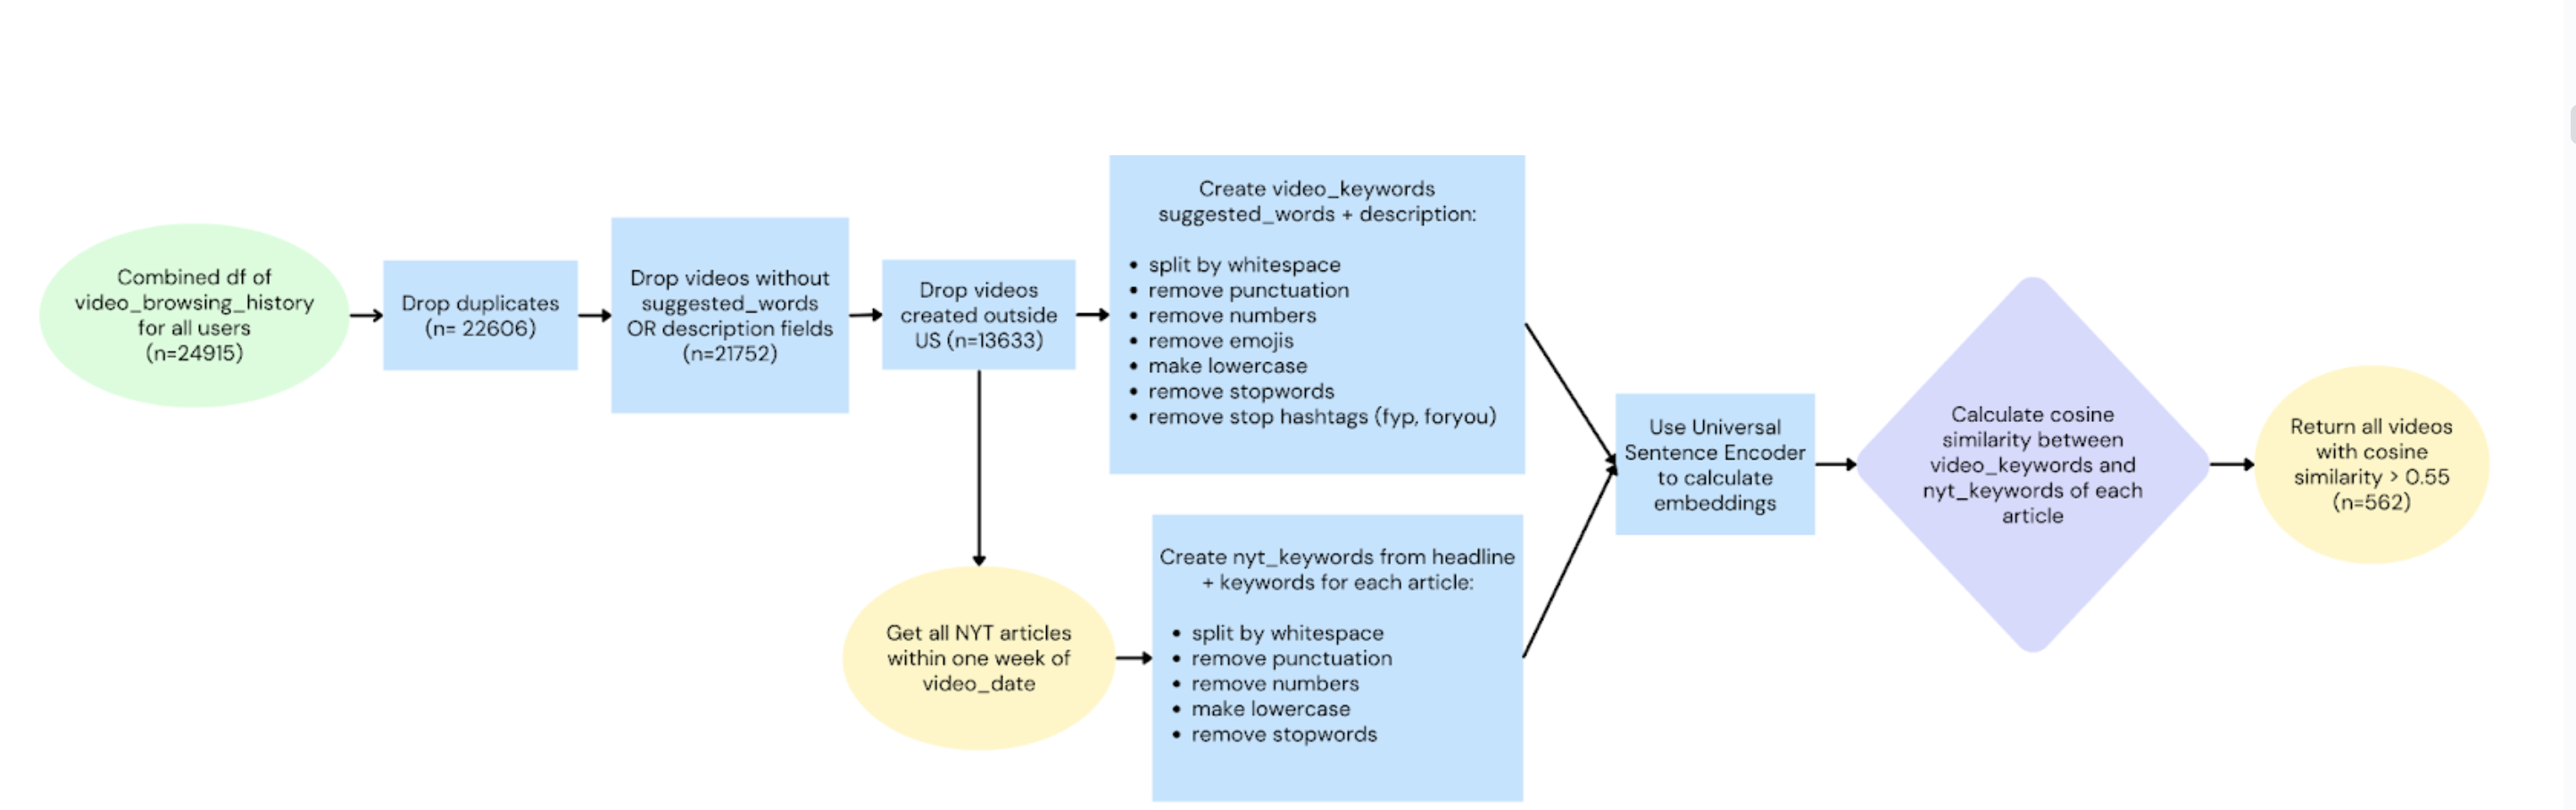
\includegraphics[width=1\linewidth]{flowchart.png} 
    \caption{The flowchart illustrates the process of filtering videos by comparing them to NYT articles. This included excluding non-US videos and those without suggested words or descriptions, generating keyword lists from both videos and NYT articles, and calculating cosine similarity using Universal Sentence Encoder embeddings. Comparisons were made between video keywords and articles published within a week of the video's upload, with videos having cosine similarity greater than or equal to 0.55 considered for transcription.}
    \label{fig:flowchart} 
  \end{figure}


{\noindent}Then, for each video, list of keywords was compiled by merging the suggested words and description, while omitting common hashtags like 'fyp' and 'for you,' which are incompatible with NYT articles. Furthermore, given the disparities between the textual content on TikTok (such as descriptions) and NYT articles, we also generated a list of keywords for each NYT article, extracted from the headline and abstract. The use of these keywords aimed to enhance the effectiveness of using cosine similarity as a metric, enabling more accurate comparisons between TikTok videos and NYT articles. \newline

{\noindent}Lastly, we utilized the Universal Sentence Encoder to compute embeddings for each list of keywords. Subsequently, for each video, cosine similarity was calculated between its keyword list and the keyword list of each NYT article published within one week of the video's upload date (three days before, the upload day, and three days after). This approach was chosen as it yielded a higher median cosine similarity (0.315) compared to solely comparing with articles on the video upload date (0.249). As a result, 516 videos with a cosine similarity of 0.55 or higher were identified for transcription.

\subsection{Transcription}
From our three filtering processes (by hashtags, by posting account, and by similarity with NYT headlines), 834 unique videos were identified as possibly related to news. Among these, 450 videos were randomly chosen for transcription. Note that we opted for sampling due to computational constraints. \newline

{\noindent}To transcribe the selected videos, the .mp4 files were downloaded through Pyktok~\cite{pyktok}. Then, each .mp4 file was passed to librosa, an audio processing package, to load and resample the audio at 16000 Hz. Afterward, Whisper, an open-source neural network specialized in automatic speech recognition, was utilized. Before the audio was passed to Whisper, it underwent processing by the Whisper processor, which includes both the feature extractor (responsible for pre-processing raw audio) and the tokenizer (used to decode transcriptions into words). Finally, the pre-processed audio was fed into the WhisperForConditionalGeneration model, which generated and returned IDs corresponding to tokens, resulting in the production of a .txt file containing the transcription for each video.\newline

\subsection{Comparison of Transcriptions to NYT articles}
From the transcribed videos, transcripts in languages other than English were excluded. Additionally, transcripts containing fewer than 18 words (the maximum NYT headline length) were filtered out. This decision was driven by the sensitivity of cosine similarity to length, as it is unlikely that transcripts with only a few words would contain substantial meaningful news content. \newline

{\noindent}Then, the remaining 227 transcriptions were compared with NYT headlines, abstracts, and lead paragraphs to assess the effectiveness of the filtering methods. Similar to the filtering step, this comparison used cosine similarity of Universal Sentence Encoder embeddings, with no pre-processing applied to either the video transcription or article headline.\newline

{\noindent}Additionally, considering the computational expense of comparing full transcripts to entire headlines, abstracts, and lead paragraphs, we sought to determine if this approach would outperform comparing keyword fields. Hence, we constructed keyword fields for the NYT articles, as detailed in Section~\ref{subsec:headline}. Similarly, we created transcription keywords by eliminating stopwords and punctuation. Subsequently, we calculated the cosine similarity between the Universal Sentence Encoders of the cleaned transcription and NYT keyword and headline data. \newline

\subsection{Qualitative Analysis}
To validate the findings regarding news-related videos identified through cosine similarity, a qualitative examination was conducted on those with the highest cosine scores. The definition of news for this analysis encompassed videos reporting or commenting on current events. Each video underwent manual analysis by three individuals, who categorized them as 'Yes,' 'No,' or 'Maybe' based on the aforementioned definition. In cases of conflicting categorizations, discussions were held to reach a consensus. Additionally, a subset of news videos pertaining to the events in Israel-Palestine were identified.\newline

\section{Results}
Recall that our primary research questions revolved around the identification of news on TikTok, the types of news showcased on the platform from October 7, 2023, to December 7, 2023, and the extent of its presence. Out of our original dataset comprising 24,915 videos, we pinpointed 834 unique videos as news-related through our three filtering methods. Subsequently, we analyzed this dataset using three approaches: (i) cosine similarity between transcripts and The New York Times, (ii) clustering, and (iii) qualitative analysis of transcripts. \newline

\subsection{Cosine Similarity Between Transcripts}
{\noindent}Figure~\ref{fig:transcription} below presents the distribution of cosine similarities computed for different groups. Across the four comparisons of the TikTok transcripts of videos identified as news-related, all yielded right-skewed cosine similarity distributions with medians ranging between 0.30 and 0.35. Notably, the median cosine similarity for comparing video keywords to NYT keywords across all videos was very similar, at 0.305. Consequently, we conclude that using cosine similarity to compare transcripts with the NYT does not appear to be any more effective in identifying news than using cosine similarity to compare video keywords to NYT keywords.\newline

\begin{figure}[h!]
    \centering
    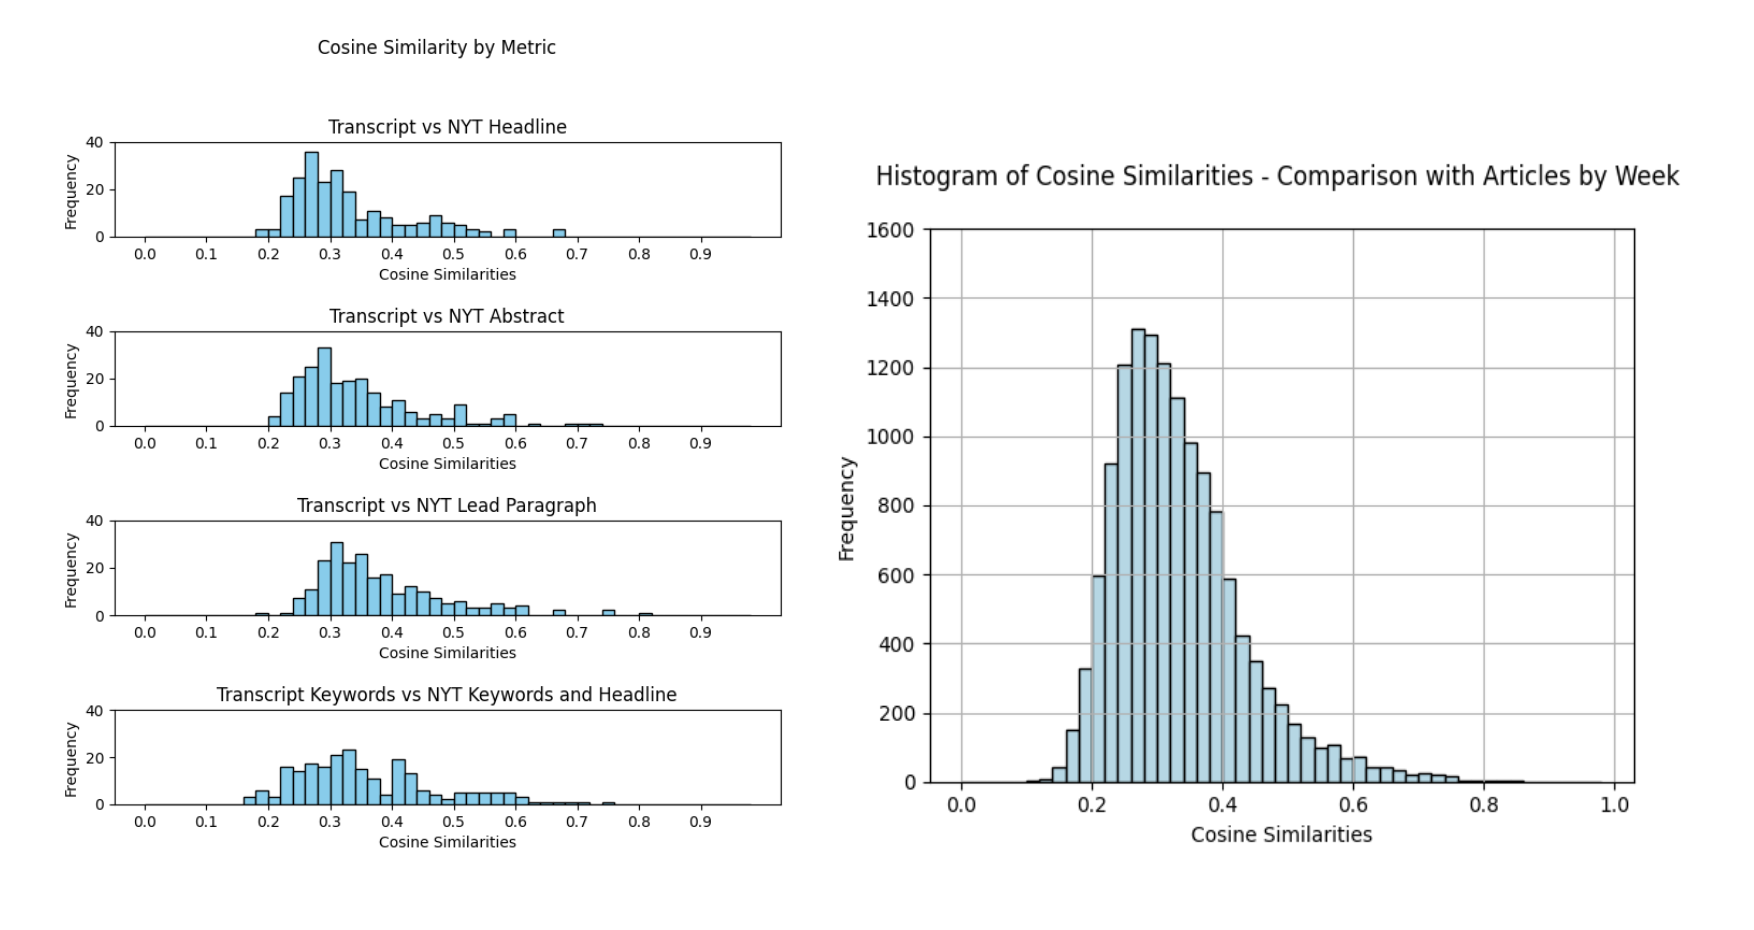
\includegraphics[width=1\linewidth]{transcription.png} 
    \caption{$Left:$ Histograms of the cosine similarities based on the video transcriptions, for videos already identified as potentially news-related. From top to bottom, their medians are: 0.304, 0.319, 0.353, and 0.332 $Right:$ Histogram of the cosine similarities between video keywords and NYT keywords, for all videos. Its median is 0.315.}
    \label{fig:transcription} 
  \end{figure}



\subsection{Clustering}
Figure~\ref{fig:clustering} depicts the results of K-Means clustering, applied to the 516 TikTok videos initially identified as news through similarity with NYT headlines. Among the eight clusters, seven exhibit cohesive themes as outlined in Appendix A2. Notably, six out of these seven clusters feature content related to cultural topics or soft news, such as 'The Hunger Games' or 'Thanksgiving.' The sole cluster related to world news is cluster 2 on Israel-Palestine, which comprises 71 videos, constituting 13.76 percent of the dataset. \newline


\begin{figure}[h!]
    \centering
    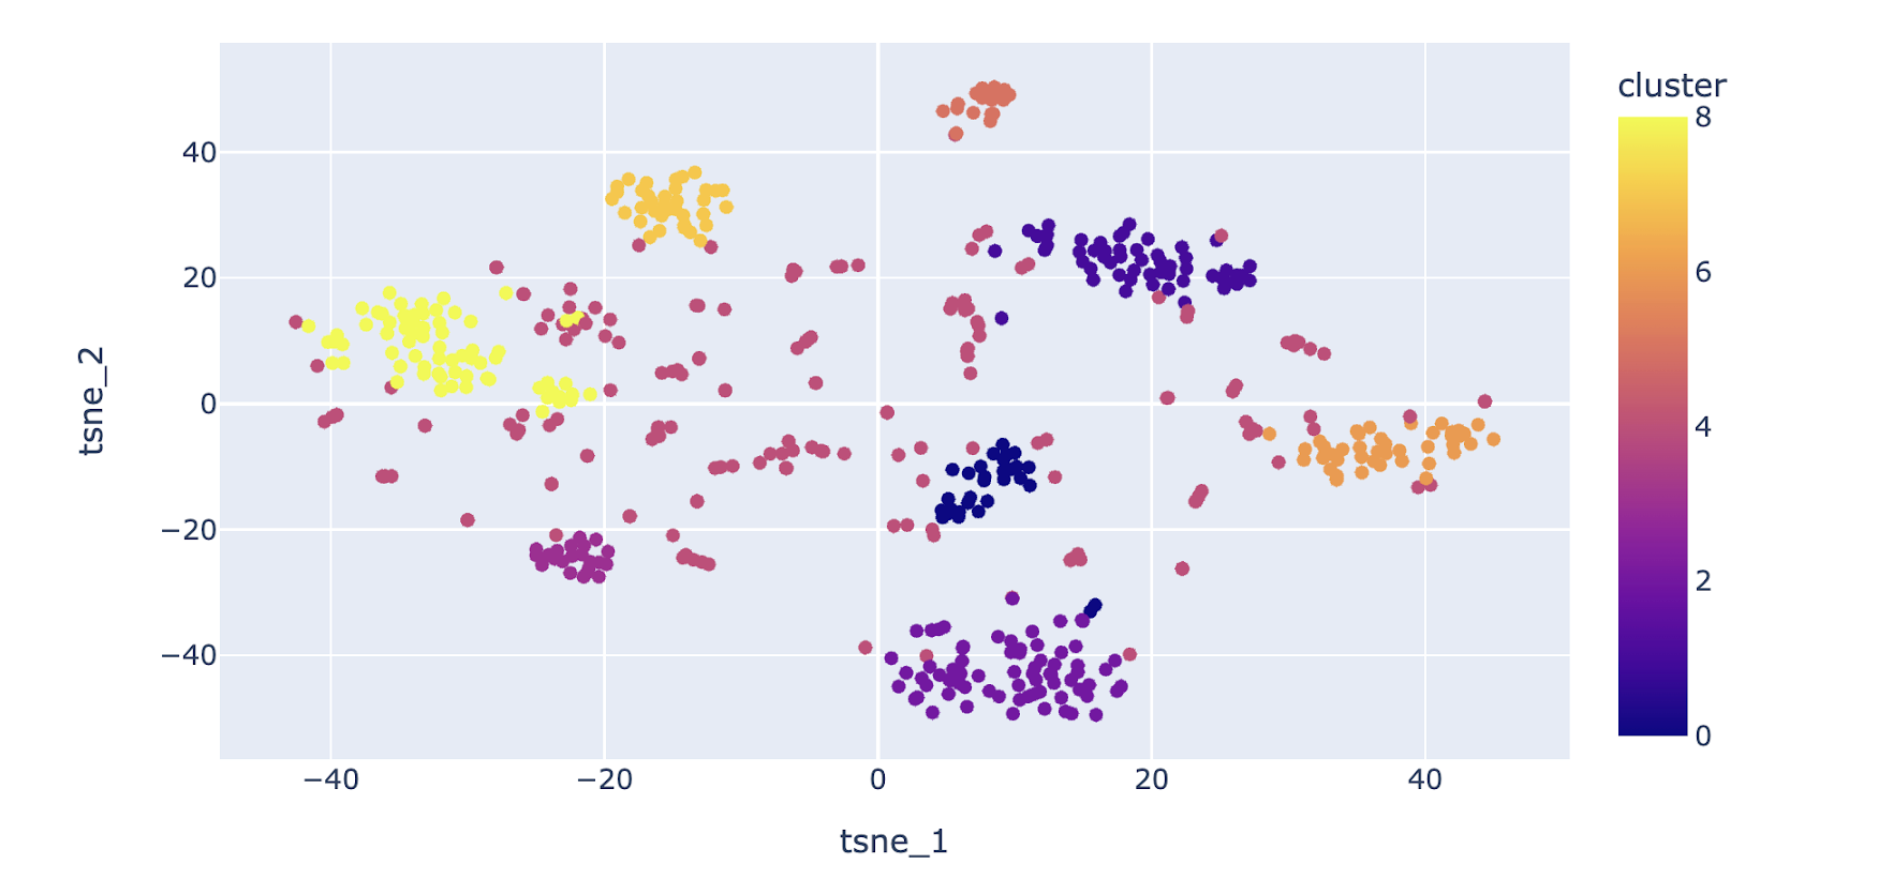
\includegraphics[width=0.9\linewidth]{cluster.png} 
    \caption{K-means Clustering of Embeddings of TikTok Videos Filtered by NYT Headline Comparison (k=8). Seven clusters are distinct and cohesive (e.g. the orange cluster 7 is about K-pop and the yellow cluster 8 is about Taylor Swift), while one cluster (the pink cluster 4) lacks a cohesive theme.}
    \label{fig:clustering} 
\end{figure}

\subsection{Qualitative Analysis}
Recall that for the qualitative examination of the transcripts, non-English content and transcripts less than 18 words long were filtered out. To human-verify whether the videos were news-related, we categorized them into three groups: 'Yes,' 'Maybe,' and 'No.' Through this process, only 72 out of the 227 videos were identified as definitively or possibly news-related, amounting to 31.7 percent. As a result, we observed that even during our selected time period, which was chosen because we hypothesized finding a substantial amount of news content, the actual news content constituted a very small percentage of our users' TikTok feeds. ~\newline

{\noindent}Notably, in the human-verified review of the transcripts, it was found that 37 videos (accounting for 51.34 percent of the sampled news-related transcripts) were related to Israel-Palestine. Although the extent of news on TikTok during our selected time period cannot be compared to another time period within the scope of this study, the current analysis suggests that a majority of the news content users received pertained to Israel-Palestine.


\section{Discussion}
{\noindent}While a considerable amount of the news content identified was related to Israel-Palestine, overall, news constituted a small portion of TikTok content during the period between October 7, 2023, and December 7, 2023. These findings could indicate that there is indeed a limited amount of news content on TikTok, which aligns with the findings of the original study\cite{hagar2023algorithmic}. However, this contrasts with a report indicating that a significant portion of TikTok users – particularly young people – claim to obtain news from the platform~\cite{pewresearch2023}. This suggests a discrepancy between how researchers and young people define and measure news. \newline

{\noindent}Through qualitative research, the difficulty of defining news became apparent. While manually tagging transcripts as news, numerous videos posed challenges in categorization. A wide-reaching definition of news was employed, yet many transcripts could have been alternatively tagged as current events-related, on-the-ground coverage, or commentary. To elaborate on the examination framework, 20 transcripts were designated as 'Maybe' news. This category encompassed mixed content, such as commentary on non-news events with a reference to world events like Israel-Palestine or on politicians. These transcripts were included in the pool due to our selection of hashtags. Additionally, among the non-news content, we observed an intriguing presence of Taylor Swift lyrics. These lyrics were initially identified as potentially news through the keyword comparison to NYT keywords, specifically resembling style and opinion articles.~\newline

{\noindent}In some cases, decisions on categorizing transcripts as news hinged on the political context at the time and the speaker's identity – information we lacked. For instance, a transcript discussing being pro-life raised uncertainty about its news value, as political opinions alone don't guarantee newsworthiness. Further context, like whether it was in response to an event, was deemed necessary. However, upon viewing the video, it became clear that the speaker was Nikki Haley, a Presidential candidate, thus qualifying it as news. This underscores the limitation that categorizing videos based solely on transcripts is not always feasible.\newline

{\noindent}Note that measurements of news – based on Hagar’s and Diakopoulus’~\cite{hagar2023algorithmic} – may have been flawed. From personal experiences, it's observed that a significant portion of news-related TikTok content originates from non-traditional news sources and is not presented in a traditional reporting style. Reflecting the egalitarian nature of TikTok, news often consists of individual users discussing current events and expressing their opinions. It's plausible that this is the type of news young people refer to when claiming to get news from TikTok. Furthermore, this form of news may not align well with metrics, as it often originates from non-traditional sources and may not be structured similarly to content from traditional news outlets, particularly in terms of language and format, as measured by cosine similarity.\newline

{\noindent}In addition to the findings, the current analysis also presents further research opportunities. Future research can extend beyond textual analysis and incorporate the visual component of the videos. Tools such as graph machine-learning techniques can uncover hidden patterns within TikTok's content ecosystem. Another promising direction is to expand upon the clustering analysis: by examining how New York Times keywords fit into existing clusters and investigating how clusters evolve over different time frames, researchers can gain insights into the dynamic nature of news-related content on TikTok. Additionally, exploring variations in clusters across different user demographics could offer valuable insights into platform usage patterns.\newline

{\noindent}To address the concern of having limited data within a constrained time frame, future work can expand the current analysis by comparing our 
selected time period to another. This comparison can focus on different time 
frames excluding incidents like Israel-Palestine to eliminate the impact on 
news types introduced by major world events. It can be used to investigate the 
association between news type distribution and significant events, providing 
insights into whether and how Israel-Palestine influenced the amount of total 
news content on TikTok.\newline

{\noindent}Finally, redefining the concept of news within the context of TikTok can also present an innovative research opportunity. As our study revealed, traditional definitions may not fully capture the diverse forms of information dissemination and user-generated content on the platform. Future investigations should consider broader conceptual frameworks that encompass the range of content types and potentially tailor the definition of news to align with individual user preferences and backgrounds. \newline

\section{Conclusion}
In our investigation into TikTok's function as a news source, it was found that despite the platform's popularity among younger demographics, news content occupies only a small fraction of users' feeds during our selected timeframe. Our analysis suggests that TikTok's algorithm assigns low priority to news dissemination, despite the global significance of events such as events relating to Israel-Palestine conflict.\newline

{\noindent}In conclusion, while this study sheds light on TikTok's role as a news source, there remains a rich area for exploration. By addressing the limitations of the current approach while embracing innovative methodologies and redefining key concepts, researchers can continue to unravel the complexities of news consumption in this growing era of TikTok.
\newpage

\section*{Appendix A1}
\addcontentsline{toc}{section}{Appendix A1}
Features collected through Pyktok. Bold features were used.
\singlespacing
\begin{itemize}
    \item {\bf video\_id}
    \item {\bf video\_timestamp}
    \item video\_duration
    \item {\bf video\_locationcreated}
    \item {\bf suggested\_words}
    \item video\_likecount
    \item video\_sharecount
    \item video\_commentcount
    \item video\_playcount
    \item {\bf video\_description}
    \item {\bf video\_is\_ad}
    \item video\_stickers
    \item author\_username
    \item author\_name
    \item author\_followercount
    \item author\_followingcount
    \item author\_heartcount
    \item author\_videocount
    \item author\_diggcount
    \item author\_verified
\end{itemize}
\newpage
\section*{Appendix A2}
\addcontentsline{toc}{section}{Appendix A2}

\begin{table}[h!]
    \centering
    \caption{Cluster Information}
    \begin{tabular}{|p{4cm}|p{2cm}|p{8cm}|}
        \hline
        \textbf{Cluster Number, (Color), Location} & \textbf{Theme} & \textbf{Video Keywords of Sample in Cluster} \\
        \hline
        0 (blue) middle & New York & ['much', 'rent', 'door', 'wont', 'close', 'nyc', 'rent', 'apartment', 'viral', 'hurricane', 'hurricanebridgitmendler'] \\ 

        \hline

        1 (bright purple) top right & Halloween & ['happy', 'halloween', 'guyssss', 'homelessant', 'homelessantmeme', 'halloween', 'halloween', 'antmeme'] \\

        \hline
        2 (purple) bottom middle & Israel-Palestine & ['day', 'ceasefire', 'yet', 'theyre', 'still', 'bmbing', 'gaza', 'youre', 'pro', 'isnotreal', 'youre', 'actually', 'sick', 'freepalestine'] \\ 
        \hline

        3 (dark pink) bottom left & The Hunger Games & ['tigris', 'hunger', 
        'games', 'lucy', 'gray', 'snow', 'hunger', 'games', 'hunger', 'games', 
        'songbirds', 'snakes', 'hunger', 'games', 'happened', 'lucy', 'gray', 
        'hunger', 'games', 'ballad', 'songbirds', 'ballad', 'songbirds', 
        'snakes', 'hunger', 'games', 'explained', 'president', 'snow', 'put', 
        'together', 'hungergames', 'balladofsongbirdsandsnakes', 'presidentsnow', 'lucygraybaird', 'endingexplained', 'movieanalysis', 'booktok'] \\ 

        \hline

        4 (pink) scattered middle & NA & ['jimmy', 'carter', 'young', 'jimmy', 
        'rosalynn', 'carter', 'hospice', 'jimmy', 'carter', 'hospice', 
        'jimmycarter', 'jimmy', 'rosalynn', 'carter', 'young', 'jimmy', 
        'carter', 'rosalynn', 'cnn', 'jimmy', 'carter', 'jimmy', 'carter', 
        'presidency', 'jimmy', 'carter', 'palestine', 'greenscreenvideo', 
        'love', 'jimmy', 'carter', 'roslynn', 'carter', 'potus'] \\ 

        \hline 
        
        5 (grapefruit) top middle & TV shows & ['informant\_part', 'antfarm', 'disney'] \\

        \hline

        6 (orange) far right &  Thanksgiving & ['best', 'mexican', 'thanksgiving', 'turkey', 'thanksgiving', 'mexican', 'turkey'] \\

        \hline
        7 (light orange) top left & K-pop & ['serious', 'would', 'think', 'finna', 'actually', 'debut', 'kpop', 'jyp', 'sm', 'yg', 'hybe', 'cube', 'blackpink', 'bts', 'twice', 'straykids', 'gidle'] \\

        \hline

        8 (yellow) & Taylor Swift & ['taylor', 'swift', 'cats', 'taylor', 'swift', 'productions', 'taylor', 'swift', 'productions', 'logo', 'taylor', 'swift', 'taylor', 'taylor', 'swift', 'performing', 'taylor', 'swift', 'tiktok', 'taylorswiftandtraviskelce', 'candace', 'owens', 'taylor', 'swift', 'margaret', 'qualley', 'taylor', 'swift', 'taylorswift']\\

        \hline
    \end{tabular}
\end{table}


\newpage 
\bibliography{paperbib}
\bibliographystyle{plain}
\end{document}
